\documentclass[12pt]{pom_thesis}
\author{Alan Antonio Peral Ortiz}
\advisor{Shahriar Shahriari}
\title{The Parks Location Problem}
\usepackage{tikz}
\usepackage{listings}

\renewcommand\lstlistingname{Function}
\renewcommand\lstlistlistingname{Software and Functions}

\usepackage{amsmath}

\usepackage{hyperref}
\hypersetup{
 	colorlinks = true,
	linkcolor = blue,
	urlcolor = magenta,
	citecolor = black,
	linktoc = page
 }
\theoremstyle{definition}
\newtheorem{definition}{Definition}[section]

\newcounter{mycount}
\newcounter{mycounter}

\tikzset{
	mygrid/.pic={
		  
\draw[step=1cm,color=gray] (-2,-2) grid (3,3);
    \node[fill=cyan] at (-1.5,2.5) {};
    \node[fill=cyan] at (0.5,2.5) {};
    \node[fill=cyan] at (-.5,.5) {};
    \node[fill=cyan] at (2.5,.5) {};
    \node[fill=cyan] at (-1.5,2.5) {};
    \node[fill=cyan] at (1.5,-.5) {};
    \node[fill=cyan] at (-1.5,-1.5) {};

\setcounter{mycount}{1}
\foreach \y in {+2.6,+1.6,.6,-.4,-1.4}
  \foreach \x in {-1.6,-0.6,.4,1.4,2.4}
    \node at (\x,\y)[anchor=north west] {\tiny\arabic{mycount}\addtocounter{mycount}{1}};


	},
	uncoloredgrid/.pic={
	\draw[step=1cm,color=gray] (-2,-2) grid (3,3);

\setcounter{mycounter}{1}
\foreach \y in {+2.6,+1.6,.6,-.4,-1.4}
  \foreach \x in {-1.6,-0.6,.4,1.4,2.4}
    \node at (\x,\y)[anchor=north west] {\tiny\arabic{mycounter}\addtocounter{mycounter}{1}};
	
	
	},
	twoparkschosengrid/.pic={
	\draw[step=1cm,color=gray] (-2,-2) grid (3,3);
   	\node[fill=cyan] at (-1.5,2.5) {};
    	\node[fill=green] at (-.5,.5) {};
     	\node[fill=cyan] at (0.5,2.5) {};
    	\node[fill=cyan] at (-1.5,2.5) {};
    	\node[fill=cyan] at (2.5,.5) {};
    	\node[fill=green] at (1.5,-.5) {};
    	\node[fill=cyan] at (-1.5,-1.5) {};
    	\node[fill=orange] at (-1.5,1.5){};
     	\node[fill=orange] at (-1.5,.5){};
     	\node[fill=orange] at (-1.5,-.5){};
     	\node[fill=orange] at (-.5,1.5){};
     	\node[fill=orange] at (-.5,-.5){};
     	\node[fill=orange] at (0.5,-.5){};
      	\node[fill=orange] at (.5,.5){};
       	\node[fill=orange] at (.5,1.5){};
       	\node[fill=orange] at (1.5,.5){};
       	\node[fill=orange] at (.5,-1.5){};
        	\node[fill=orange] at (1.5,-1.5){};
         \node[fill=orange] at (2.5,-1.5){};
         \node[fill=orange] at (2.5,-.5){};
   
	\setcounter{mycount}{1}
	\foreach \y in {+2.6,+1.6,.6,-.4,-1.4}
  	\foreach \x in {-1.6,-0.6,.4,1.4,2.4}
    	\node at (\x,\y)[anchor=north west] {\tiny\arabic{mycount}\addtocounter{mycount}{1}};
	
	},
	popgrid/.pic = {
	\draw[step=1cm,color=gray] (-2,-2) grid (3,3);
   	\node[fill=cyan] at (-1.5,2.5) {};
    	\node[fill=cyan] at (-.5,.5) {};
     	\node[fill=cyan] at (0.5,2.5) {};
    	\node[fill=cyan] at (-1.5,2.5) {};
    	\node[fill=cyan] at (2.5,.5) {};
    	\node[fill=cyan] at (1.5,-.5) {};
    	\node[fill=cyan] at (-1.5,-1.5) {};
    	\node at (-1.5,1.5){50};
     	\node at (-1.5,.5){40};
     	\node at (-1.5,-.5){35};
     	\node at (-.5,2.5){200};
     	\node at (-.5,1.5){100};
     	\node at (-.5,-.5){50};
     	\node at (0.5,-.5){140};
      	\node at (.5,.5){150};
       	\node at (.5,1.5){150};
       	\node at (1.5, 1.5){160};
       	\node at (2.5, 1.5){20};
       	\node at (2.5,2.5){30};
       	\node at (1.5,2.5){200};
       	\node at (1.5,.5){140};
       	\node at (-.5,-1.5){60};
       	\node at (.5,-1.5){95};
        	\node at (1.5,-1.5){85};
         \node at (2.5,-1.5){60};
         \node at (2.5,-.5){90};
   
	\setcounter{mycount}{1}
	\foreach \y in {+2.6,+1.6,.6,-.4,-1.4}
  	\foreach \x in {-1.6,-0.6,.4,1.4,2.4}
   	\node at (\x,\y)[anchor=north west] {\tiny\arabic{mycount}\addtocounter{mycount}{1}};
	},
	bigexample/.pic = {
	
	\draw [step=0.5cm, very thin, color=black, solid] (0, 0) grid (7.5, 5);
	% row 1 pop
	\node at (0.25,4.75){\footnotesize 50};
	\node at (0.75,4.75){\footnotesize 55};
	\node at (1.75,4.75){\footnotesize 40};
	\node at (2.25,4.75){\footnotesize 60};
	\node at (2.75,4.75){\footnotesize 85};
	\node at (3.25,4.75){\footnotesize 65};
	\node at (3.75,4.75){\scriptsize 120};
	\node at (4.25,4.75){\scriptsize 105};
	\node at (4.75,4.75){\footnotesize 95};
	\node at (5.25,4.75){\footnotesize 85};
	\node at (6.25,4.75){\footnotesize 65};
	\node at (6.75,4.75){\footnotesize 45};
	% row 2 pop
	\node at (0.75,4.25){\footnotesize 50};
	\node at (1.25,4.25){\footnotesize 45};
	\node at (1.75,4.25){\footnotesize 60};
	\node at (2.25,4.25){\scriptsize 110};
	\node at (2.75,4.25){\scriptsize 120};
	\node at (3.25,4.25){\footnotesize 95};
	\node at (3.75,4.25){\scriptsize 110};
	\node at (4.75,4.25){\scriptsize 100};
	\node at (5.25,4.25){\footnotesize 65};
	\node at (5.75,4.25){\footnotesize 75};
	\node at (6.25,4.25){\footnotesize 40};
	\node at (6.75,4.25){\footnotesize 45};
	\node at (7.25,4.25){\footnotesize 30};
	% row 3 pop
	\node at (0.25,3.75){\footnotesize 80};
	\node at (0.75,3.75){\footnotesize 75};
	\node at (1.25,3.75){\footnotesize 55};
	\node at (1.75,3.75){\footnotesize 70};
	\node at (2.25,3.75){\scriptsize 105};
	\node at (2.75,3.75){\scriptsize 130};
	\node at (3.25,3.75){\scriptsize 115};
	\node at (4.25,3.75){\scriptsize 105};
	\node at (4.75,3.75){\scriptsize 115};
	\node at (5.25,3.75){\footnotesize 80};
	\node at (5.75,3.75){\footnotesize 50};
	\node at (6.25,3.75){\footnotesize 65};
	\node at (6.75,3.75){\footnotesize 50};
	% row 4 pop
	\node at (0.25,3.25){\scriptsize 165};
	\node at (1.25,3.25){\footnotesize 65};
	\node at (2.25,3.25){\footnotesize 65};
	\node at (2.75,3.25){\footnotesize 80};
	\node at (3.25,3.25){\footnotesize 95};
	\node at (3.75,3.25){\scriptsize 110};
	\node at (4.25,3.25){\scriptsize 105};
	\node at (5.25,3.25){\footnotesize 70};
	\node at (5.75,3.25){\footnotesize 55};
	\node at (6.25,3.25){\footnotesize 45};
	\node at (7.25,3.25){\footnotesize 25};
	% row 5 pop
	\node at (0.25,2.75){\scriptsize 225};
	\node at (0.75,2.75){\scriptsize 200};
	\node at (1.25,2.75){\footnotesize 70};
	\node at (1.75,2.75){\footnotesize 75};
	\node at (2.25,2.75){\scriptsize 100};
	\node at (3.25,2.75){\scriptsize 100};
	\node at (3.75,2.75){\scriptsize 105};
	\node at (4.25,2.75){\scriptsize 120};
	\node at (4.75,2.75){\scriptsize 105};
	\node at (5.25,2.75){\footnotesize 55};
	\node at (6.25,2.75){\footnotesize 20};
	\node at (6.75,2.75){\footnotesize 25};
	\node at (7.25,2.75){\footnotesize 15};
	% row 6 pop
	\node at (0.25,2.25){\scriptsize 250};
	\node at (0.75,2.25){\scriptsize 120};
	\node at (1.75,2.25){\footnotesize 85};
	\node at (2.25,2.25){\scriptsize 105};
	\node at (2.75,2.25){\scriptsize 100};
	\node at (3.25,2.25){\scriptsize 110};
	\node at (3.75,2.25){\footnotesize 70};
	\node at (4.25,2.25){\footnotesize 80};
	\node at (4.75,2.25){\footnotesize 70};
	\node at (5.25,2.25){\footnotesize 65};
	\node at (5.75,2.25){\footnotesize 50};
	\node at (6.25,2.25){\footnotesize 15};
	\node at (6.75,2.25){\footnotesize 5};
	\node at (7.25,2.25){\footnotesize 10};
	% row 7 pop
	\node at (0.25,1.75){\scriptsize 200};
	\node at (0.75,1.75){\scriptsize 100};
	\node at (1.25,1.75){\scriptsize 180};
	\node at (1.75,1.75){\scriptsize 155};
	\node at (2.25,1.75){\scriptsize 125};
	\node at (2.75,1.75){\scriptsize 105};
	\node at (3.25,1.75){\footnotesize 80};
	\node at (4.25,1.75){\footnotesize 95};
	\node at (4.75,1.75){\footnotesize 75};
	\node at (5.25,1.75){\footnotesize 40};
	\node at (5.75,1.75){\footnotesize 45};
	\node at (6.25,1.75){\footnotesize 35};
	\node at (7.25,1.75){\footnotesize 15};
	% row 8 pop
	\node at (0.25,1.25){\scriptsize 250};
	\node at (1.75,1.25){\scriptsize 145};
	\node at (2.75,1.25){\scriptsize 235};
	\node at (3.25,1.25){\scriptsize 100};
	\node at (3.75,1.25){\footnotesize 80};
	\node at (4.25,1.25){\scriptsize 135};
	\node at (4.75,1.25){\footnotesize 95};
	\node at (5.25,1.25){\footnotesize 70};
	\node at (6.25,1.25){\footnotesize 50};
	\node at (6.75,1.25){\footnotesize 45};
	\node at (7.25,1.25){\footnotesize 20};
	% row 9 pop
	\node at (0.25,0.75){\scriptsize 300};
	\node at (1.25,0.75){\scriptsize 265};
	\node at (1.75,0.75){\scriptsize 205};
	\node at (2.25,0.75){\scriptsize 235};
	\node at (2.75,0.75){\scriptsize 505};
	\node at (3.25,0.75){\scriptsize 500};
	\node at (3.75,0.75){\scriptsize 245};
	\node at (4.25,0.75){\scriptsize 175};
	\node at (4.75,0.75){\footnotesize 80};
	\node at (5.25,0.75){\footnotesize 85};
	\node at (5.75,0.75){\footnotesize 65};
	\node at (6.25,0.75){\footnotesize 30};
	\node at (7.25,0.75){\footnotesize 25};
	% row 10 pop
	\node at (0.25,0.25){\scriptsize 305};
	\node at (0.75,0.25){\scriptsize 255};
	\node at (1.25,0.25){\scriptsize 275};
	\node at (1.75,0.25){\scriptsize 215};
	\node at (2.25,0.25){\scriptsize 225};
	\node at (2.75,0.25){\scriptsize 400};
	\node at (3.25,0.25){\scriptsize 405};
	\node at (3.75,0.25){\scriptsize 410};
	\node at (4.25,0.25){\scriptsize 500};
	\node at (4.75,0.25){\scriptsize 305};
	\node at (5.75,0.25){\footnotesize 45};
	\node at (6.25,0.25){\footnotesize 50};
	\node at (6.75,0.25){\footnotesize 40};
	\node at (7.25,0.25){\footnotesize 30};

	% candidate parcels
	\filldraw[fill=cyan, draw=black] (7, 4.5) rectangle (7.5, 5);
	\filldraw[fill=cyan, draw=black] (5.5, 4.5) rectangle (6, 5);
	\filldraw[fill=cyan, draw=black] (1, 4.5) rectangle (1.5, 5);
	\filldraw[fill=cyan, draw=black] (0, 4) rectangle (0.5, 4.5);
	\filldraw[fill=cyan, draw=black] (4, 4) rectangle (4.5, 4.5);
	\filldraw[fill=cyan, draw=black] (3.5, 3.5) rectangle (4, 4);
	\filldraw[fill=cyan, draw=black] (7, 3.5) rectangle (7.5, 4);
	\filldraw[fill=cyan, draw=black] (0.5, 3) rectangle (1, 3.5);
	\filldraw[fill=cyan, draw=black] (1.5, 3) rectangle (2, 3.5);
	\filldraw[fill=cyan, draw=black] (4.5, 3) rectangle (5, 3.5);
	\filldraw[fill=cyan, draw=black] (6.5, 3) rectangle (7, 3.5);
	\filldraw[fill=cyan, draw=black] (2.5, 2.5) rectangle (3, 3);
	\filldraw[fill=cyan, draw=black] (5.5, 2.5) rectangle (6, 3);
	\filldraw[fill=cyan, draw=black] (1, 2) rectangle (1.5, 2.5);
	\filldraw[fill=cyan, draw=black] (3.5, 1.5) rectangle (4, 2);
	\filldraw[fill=cyan, draw=black] (6.5, 1.5) rectangle (7, 2);
	\filldraw[fill=cyan, draw=black] (0.5, 1) rectangle (1, 1.5);
	\filldraw[fill=cyan, draw=black] (1, 1) rectangle (1.5, 1.5);
	\filldraw[fill=cyan, draw=black] (2, 1) rectangle (2.5, 1.5);
	\filldraw[fill=cyan, draw=black] (5.5, 1) rectangle (6, 1.5);
	\filldraw[fill=cyan, draw=black] (0.5, 0.5) rectangle (1, 1);
	\filldraw[fill=cyan, draw=black] (6.5, 0.5) rectangle (7, 1);
	\filldraw[fill=cyan, draw=black] (5, 0) rectangle (5.5, 0.5);
	
	}
}



\begin{document}
\lstset{
	literate={``}{\textquotedblleft}1,
    	deletestring=[b]",
    	showstringspaces=false,
	belowcaptionskip = 15pt,
	belowskip = 15pt
}


\maketitle

\begin{abstract}We take a look at the multiobjective facility location problem of park placement in the city of Bogot\'{a}, Colombia. We begin with an introduction to operations research, explore the notion of community based operations research and multiobjective optimization problems, and then introduce a simplified model based on our real scenario. We work up from this example to construct our final model. We then examine the computer program I developed to solve our mathematical model.
\end{abstract}

\pagenumbering{roman}
\tableofcontents
\lstlistoflistings

\newpage
\pagenumbering{arabic}
% this is how you begin a chapter:
% the label is so that you can refer to it later
\begin{chapter}{Introduction} \label{intro}

%
% 1.1
%
\section{The Parks Location Problem} \label{intro-parks-problem}

	In urban areas and large cities, the presence of public parks, green spaces, and other recreational facilities has been associated with a significant improvement in quality of life, mental health, and general wellbeing \cite{bogota}. Knowing this, the city of Bogot\'{a} (Colombia), one of the largest cities in Latin America with a population of about eight million that is expected to reach ten million by 2025, has implemented a number of changes that include the recovery of public spaces and the improvement of public parks \cite{bogota}. 
	
	In 2006, the mayor and city council of Bogot\'{a} threw their support behind a sports and recreation master plan for the city. This plan indicated that by 2019 the city must reach a minimum level of $2.71$  $\textrm{m}^2$ of neighborhood park area per resident. It then became the \textit{Instituto Distrital de Recreaci\'{o}n y Deporte} (IDRD), or Recreation and Sports Institute of Bogot\'{a}'s job to implement the master plan. As such, the IDRD was faced with a monumental challenge: they had to execute the construction of numerous new parks and revitalize dilapidated public spaces in a manner that balanced the differing geographic, social, and economic needs of the city. 
	
	Their task turned out to be well-suited to modeling techniques, particularly as an optimization problem in the vein of operations research problems. Due to the many requirements of the project and the nature of the problem, this problem was an ideal candidate to tackle with one of the many optimization techniques existing in operations research.
%
% 1.2
%
\section{What is Operations Research?}

We begin with a brief history of Operations Research (OR), which is fundamentally the science of decision making. With this more informal perspective, we can deduce that OR has existed in some way, shape, or form for as long as humans have had to make decisions. As a modern discipline, however, OR has its roots in the Soviet political economy as well as the British war effort of World War II \cite{or-timeline}.
%
% 1.2.1
%
\subsection{The Soviet Political Economy}
	In February of 1921, the Bolsheviks established the State General Planning Commission (Gosplan for short) and set out to implement a unified economic plan for the national economy \cite{socialist-planning}. This generally marks the beginning of the Soviet experiment in central planning of the economy.  In 1928, L.P. Yushkov described what became a central problem of theory of the optimally functioning socialist economy. He was interested in creating a system of planning that would provide the `semi-automatic optimality' of the development of the national economy, combining optimal national economic development with maximal operational independence for the separate parts of the economic system \cite{planning-problems}. 
	
	The Gosplan also developed a Five-Year Plan, adopted in 1929, to help chart the course for the economy. For various reasons, including in part the ambitious goals set by their plan, the next five years were dominated by crisis, and it wasn't until after this period that they achieved a more stable economic system \cite{socialist-planning}. However, by the time the Great Depression in the United States was in full swing, the Soviet economy was in much better shape, growing healthily and retaining its stability. In fact, the Soviet economy had a remarkable number of achievements: it vastly increased the output of key industrial sectors (like oil and steel), it produced the huge number of weapons necessary to win World War II, it provided full employment, it produced the world's first earth satellite, and it invested heavily in human capital \cite{socialist-planning}.
	
	The relevance of the Soviet economy with respect to Operations Research can be established by realizing that in planning the central economy, the Soviet researchers were faced with (essentially) a giant optimization problem. They had millions of outputs (raw materials), and had to optimize for the production of an incredibly high number of outputs (consumer goods). This was an incredibly difficult task and influenced the use and development of operations research in the Soviet Union.
	
	In 1939, the Russian mathematician and economist Leonid V. Kantorovich published \textit{Mathematical Methods of Organization and Planning Production} in which he mathematically described a production assignment problem that was the first instantiation of a liner program \cite{or-timeline}. He proposed a computational procedure to solve the problem, and mentioned that this structure could be used to tackle problems in oil refining, utilization of fuel types, minimization of scrap, construction planning, the distribution of freight over a network, and the optimal distribution of arable land to different crops. Kantorovich established himself as a pioneer in the theory and use of linear programming.\\
%
% 1.2.2
%
\subsection{The Research of Military Operations}	
	Now, in the year 1934 as Nazi Germany denounced the Treaty of Versailles, Britain sensed the threat and raced to strengthen its defenses. By the following year, radar had been developed and was capable of effectively detecting enemy aircraft, although its utility was stringent on its ability for integration with the existing defense systems: ground observers, interceptor aircraft, and antiaircraft artillery positions. The first task of the newly formed operational research group was to use scientific, rigorous processes to develop a system for the incorporation of radar into existing infrastructure, which was far from the more well-defined mathematical processes that exist today. However, this integrated radar-based air defense system increased the probability of intercepting an enemy aircraft by a factor of ten \cite{us-army}.	
	
	 Soon, the usage of OR spread to investigate other problems, and in 1940 was even called upon to influence high-level strategic policy when the French requested additional RAF fighter support. Churchill was inclined to acquiesce to the request, but an OR team showed that sending more RAF fighters would weaken Britain beyond recovery in the face of a German attempt to invade Britain \cite{us-army}. Churchill was convinced by their presentation, and so he did not send the additional aircraft, preserving the pilots and aircrafts for the Battle of Britain instead. This decision, along with the incorporation of radar, contributed significantly to Britain's victory in the Battle of Britain \cite{us-army}. 
	
	Another significant accomplishment of OR analysts involved the work of deciding upon depth charge settings for bombs. Their work in this field led to an immediate improvement on aerial attacks of German submarines, with estimates of the increased efficiency ranging from 400 to 700 percent \cite{us-army}. Other work included reducing the number of artillery rounds required to down one German aircraft  from twenty thousand in the summer of 1941 to merely four thousand the following year \cite{us-army}.
	From the British, this discipline spread to the Americans, where it was also used in the war effort.
	
	This specific need to allocate scarce resources to military operations in an effective manner became so advantageous that the British and US militaries both adopted the process of performing \textit{research on} (military) \textit{operations}. In essence, the goal was to make the war machine more efficient, and they succeeded. They developed effective ways to use the new radar technology and came up with better ways to manage convoys and conduct antisubmarine operations \cite{intro-or}.	
	
	The success that OR saw in the war then encouraged interest in non-military applications of the field, and over the course of many years, OR became an indispensable tool for any major enterprise. Today, problems in OR range from production planning, to logistics and distribution of goods, to call center management, to portfolio optimization, and more \cite{community-or}.
% more intro shit

	A cursory glance at a variety of introductory textbooks will reveal that there is a certain focus on private sector applications of the field \cite{community-or}. These applications tend to be primarily concerned with profit maximization and other aspects of running a business. While these problems can provide for some interesting mathematical formulations, the field's full range of capabilities is not adequately reflected in these industry-centric perspectives.
	
	There is a subfield of the discipline called Community Based Operations Research, which seeks to shift the focus of OR from profit maximization or cost-reduction to improving the quality of life within a community. One of the advocates of the field and of this lens that focuses on people as opposed to money is Michael P. Johnson, who compiled a textbook containing a variety of case studies that can constitute ``Community-Based Operations Research." 
	
	One of these case studies presented is the problem of park location in Bogot\'{a}, Colombia. But before we delve more into it, we will explore the idea of Community Based Operations Research.

%
% 1.3
%	
\section{Community Based Operations Research}
As previously mentioned, Community Based Operations Research (CBOR) is a subfield of OR that seeks to center human experiences. This is an important position for the field to take, considering that much of our lives are defined by things provided by not-for-profit means, such as education, public safety, human and social services, community and economic development, and environmental conservation and preservation. Michael P. Johnson notes, ``We refer to OR/MS applications that address provision of goods and services, or prescribe social policy actions, for which stakeholders are defined, in a spatial or social sense, as localized, or who are considered disadvantaged or underserved, or for which issues of equity or social influence are important considerations, as examples of \textit{community-based operations research}" \cite{community-or}. Instead of furthering inequality by helping maximize a corporation's profits, it is possible for OR to be applied to local community issues or other larger problems in a way that benefits exploited and disenfranchised groups of people. 

	The arguments in favor of CBOR, in fact, concern both scholarship and the possibility of (generally speaking) improving lives. There is a vital importance of space, place, and community in policy design and service delivery that CBOR seeks to address. Furthermore, CBOR centers disadvantaged, underrepresented, or underserved populations, seeking to engage them as equal partners in joint projects and allowing them the agency and autonomy to determine their own path forward. Lastly, the international and transnational applications of these methods extend beyond the use of traditional models in a US-based context, increasing their importance and significance substantially.
	
	It turns out that the methods used in CBOR vary widely, ranging from more traditional instances of prescriptive math models to combinations of qualitative and quantitative methods that may have a lot of common ground with disciplines such as urban development and public health, among others. CBOR is a cross-disciplinary field with many future avenues for research and with many fundamental questions about it that have yet to be addressed. For example, is there a way to practice OR that balances quantitative approaches dominant in US-style practice with more critical and subjective approaches to decision modeling, accommodating qualitative and mixed-methods? Is ``rigorous" OR compatible with our values of social change and justice? Is there a theory of CBOR to be developed? Can CBOR research ever hope to be represented in the most prestigious research journals to influence the understanding of CBOR within the larger OR discipline? \cite{community-or} And in fact, do some of these questions even matter?
	
	Historically, there have been three trends in OR that have precipitated major disagreements regarding the role of OR in society \cite{community-or}. The first trend concerned the public service oriented OR  of the 1960s. In 1966, for example, MIT held the Operations Research in Public Affairs Program, which as the name implies was oriented towards public service projects. The second trend occurred with the institutionalization of OR within private-sector companies, and so OR transitioned from a transformational technology to one increasingly focused on mathematical analysis and incremental gains in efficiency. The third trend encompassed societal disenchantment with quantitative methods that promised much but delivered little (especially considering the Vietnam War and the social unrest of the times). Some of these trends were embodied in the long-ongoing disagreements between US-style operations researchers and UK-style researchers, with the US-style being defined by a mathemtical and problem-focused approach while the UK style approach was more critical and closely examined the roles of power, class, and community in defining problems amenable to OR methods \cite{community-or}.

	In summation, there is a lot of aspects about CBOR that still need to be defined, and unfortunately it still has a long way to go before it is truly respected as a field, but it could stand to fundamentally change the way we consider optimization problems in certain areas.
%
% 1.4
%
\section{Multiobjective Optimization Problems}
As the name implies, multiobjective optimization problems differ from single objective optimization problems in the number of objectives that are being optimized. In business, management, engineering, and (especially) community-oriented problems, there can be multiple conflicting objectives that need to be satisfied. Traditionally, such problems have been tackled by converting all objectives into a single objective function through the aggregation of the objectives into a weighted function \cite{pareto-mo}. Another way that multiobjective optimization problems have been typically tackled is by transforming all but one objective into constraints, and then optimizing one lone objective. 

	These types of approaches have limitations. They require \textit{a priori\footnote{adj. theoretically-deduced, not proceeding from observation or experience.}} knowledge about the importance of the objectives as well as limit the objectives when they are turned into constraints. The aggregated function approach also only leads to one solution, which you then have no easy way of comparing it to other potential solutions. Furthermore, the trade-offs between the objectives cannot be easily quantified, and a solution may not be attainable at all. These limitations make it very difficult to apply these methods in more complex systems, especially because we are dealing with multiobjective problems.
	
	Generally speaking, multiobjective problems tend to be much harder to solve than single objective problems because multiobjective problems do not have one, unique solution. Instead, there exists a set of acceptable trade-off optimal solutions which is called the Pareto front \cite{pareto-mo}. In many multiobjective problems, we will be working with people who have domain specific knowledge and who will be better positioned to make choices about the final solution. These people are referred to as the decision makers (because their input is invaluable in the model formulation process). When the decision makers have access to the Pareto set of solutions, it allows them to see a wide range of options and make informed decisions \cite{pareto-mo}. 
	
	A modern approach to generating the Pareto front involves the use of evolutionary computing, which emulates the biological evolution process, where survival of the fittest (solution) is the law of the land \cite{pareto-mo}. There are a variety of algorithms that utilize this framework: the multiobjective genetic algorithm, the Non-dominated Sorting Genetic Algorithm, the Niched Pareto Genetic Algorithm, the Strength Pareto Evolutionary Algorithm, and the Multi Objective Particle Swarm Optimization, among others. These modern methods allow for the concurrent exploration of the Pareto front, and can therefore generate multiple solutions in a single run-through. The performance of these algorithms does degrade as the number of objectives increases, however, since there do not exist computationally efficient methods to perform pareto ranking \cite{pareto-mo}. 
	
	For our purposes, we utilize the $\epsilon$-constraints approach, which we will describe in detail in \autoref{solution-strat}. Compared to the evolutionary based algorithms, this is a relatively simple technique, but it is computationally intensive as well. With this information in hand we are now ready to dive into our problem.
%
% 1.5
%
\section{Road Map}
In the next chapter we will begin to talk about the park location formulation with more depth and clarity. We will make some simplifying assumptions and construct a less complicated model, building it up as we progress and constructing a more robust model. We will then move onto the real world scenario, explaining any new concerns that arise and examining how these are incorporated into the model. The third chapter will be more technical as we delve into the Python program I have coded to solve our simplified versions of the model.
	% you should close a chapter before beginning a new one!
\end{chapter}

%
%
% Chapter 2
%
%
\begin{chapter}{A Look at the Model}
In this chapter I present a simplified version of the model. We will take a look at some simpler examples and gradually increase the complexity of our example until we arrive at the one presented in the paper. 
%
% 2.1
%
\section{A Simplified Model} 
We first look at a model that has been adapted from a real model developed by researchers working in Bogot\'{a}. This simpler version of the model will help us understand the more complex project and can serve as a learning tool to both introduce the concept of multiobjective optimization and community based operations research.
%
% 2.1.1
%
\subsection{Setting up the Problem} \label{setting-up-problem}

We begin with a $5\times5$ grid, which will represent our simplified fictional city. Each block represents a plot of land, which might either be empty or occupied. If it is occupied, this means that there are people living on the block. Otherwise, the lot is empty and it is a candidate parcel, to potentially be turned into a park. We number each block from one to $25$, and we have colored every candidate parcel cyan. We want to build one park, and so we can choose from amongst all the cyan parcels. This is shown in \autoref{fig:grid1}. We note that every lot is the same size. We also define the service area of the candidate parcels to consist of all the populated blocks adjacent and diagonal to the candidate parcel. For example, candidate parcel one's service area will consist of the set $\{2,6,7\}$. In other words, if we built a park on candidate parcel one, then the visitors would be from \textbf{only} those three surrounding lots. The first question we are interested in asking then becomes: 
\begin{center}
\textbf{Which candidate parcel will maximize the geographical coverage, as measured by the service area of the parcel?}
\end{center}
\begin{figure}
 \centering
 \caption{Our $5\times 5$ grid city}
 \label{fig:grid1}
 \begin{tikzpicture}[every node/.style={minimum size=1cm-\pgflinewidth}]
  \pic{mygrid};
\end{tikzpicture}
\end{figure}
In this example, it is possible to answer our question after merely observing the grid. Candidate parcel 12 would result in the highest number of lots served with 8. We now move on to defining a certain number of sets and variables so that we can present a mathematical formulation of the problem. \newline 
	
	We first let $\mathcal{J}$ be the set of all blocks that would benefit from the construction of a new park. Looking back to \autoref{fig:grid1}, we see that $\mathcal{J} = \{ 2,4,6,7, \dots, 22, 23, 24, 25\}$. The candidate parcels have not been included in this set, and in this case we note that lot five is not included in $\mathcal{J}$ either because it is outside the service area of every candidate parcel. We also then define the set $\mathcal{I}$ to be the set of candidate parcels. In our case, $\mathcal{I} = \{ 1,3,12,15,19,21\}$. We finally define the set $\mathcal{W}_j$ for $j \in \mathcal{J}$, which consists of all the candidate parcels that service block $j$. In our example, $\mathcal{W}_7 = \{1,3,12\}$. \newline
	
	We now define $z_j$ as a binary decision variable, taking on the value 1 if block $j \in \mathcal{J}$ is covered by at least one park, and 0 otherwise. So if we decided to build a park on candidate parcel 21, then $z_{16} = z_{17} = z_{22} = 1$, and for every other possible value of $j$ we would have $z_j = 0$. We also define the binary decision variable $y_i$, which will take on value 1 if candidate parcel $i$ is selected to become a park, and 0 otherwise. If we turned candidate parcel 21 into a park, then $y_{21} = 1$. We can now formulate our initial model:
\begin{align*}
\textrm{max } f_1 &= \sum_{j \in \mathcal{J}} z_j \\
\textrm{subject to } z_j &\leq \sum_{i \in \mathcal{W}_j} y_i, j \in \mathcal{J}\\
\left|\mathcal{W}_j\right|z_j &\geq \sum_{i \in \mathcal{W}_j} y_i, j \in \mathcal{J} \\
p_{max} &\geq \sum_{i \in \mathcal{I}} y_i \\
z_j &\in \{0,1\}, j \in \mathcal{J} \\
y_i &\in \{0,1\}, i \in \mathcal{I}
\end{align*}

	Our objective function seeks to maximize the geographical coverage of the potential parks to be built. The first constraint guarantees that if block $j$ is covered, then at least one parcel servicing it has been selected as a park. So if block 2 is covered in \autoref{fig:grid1}, then either candidate parcel 1 or candidate parcel 3 should have been selected to become a park. Conversely, the second constraint guarantees that if block $j$ is not covered, then none of the candidate parcels servicing it should be selected as parks. While I have referred to these first two constraints as being one individual constraint each, the observation can be made that they must be satisfied for all values of $j \in \mathcal{J}$, meaning that each constraint must be repeated $|\mathcal{J}|$ times. \\ \\
	\begin{figure}
	\centering
	\caption{Fully expanded model}
	\label{expandedmodel}
	
		\begin{align*}
		\textrm{max } f_1 &= z_2 + z_4 + z_6 + z_7 + z_8 + z_9 + z_{10} + z_{11} + z_{13} + z_{14} \\
		&+ z_{16} + z_{17} + z_{18} + z_{20} + z_{22} + z_{23} + z_{24} + z_{25}
		\end{align*}
	\begin{equation*}
	\begin{aligned}[c]
	\textrm{subject to } z_2 &\leq y_1 + y_3 \\
	z_4 &\leq y_3\\
	z_6 &\leq y_1 + y_{12}\\
	z_7 &\leq y_1 + y_3 +y_{12}\\
	z_8 &\leq y_3 + y_{12} \\
	z_9 &\leq  y_3 + y_{15} \\
	z_{10} &\leq y_{15} \\
	z_{11} &\leq y_{12} \\
	z_{13} &\leq y_{12} + y_{19} \\
	z_{14} &\leq y_{15} + y_{19} \\
	z_{16} &\leq y_{12} + y_{21} \\
	z_{17} &\leq y_{12} + y_{21} \\
	z_{18} &\leq y_{12} + y_{19} \\
	z_{20} &\leq y_{15} + y_{19} \\
	z_{22} &\leq y_{21} \\
	z_{23} &\leq y_{19} \\
	z_{24} &\leq y_{19} \\
	z_{25} &\leq y_{19} 
	\end{aligned}
	\qquad \qquad \qquad
	\begin{aligned}[c]
	|W_2|z_2 &\geq y_1 + y_3 \\
	|W_4|z_4 &\geq y_3 \\
	|W_6|z_6 &\geq y_1 + y_{12} \\
	|W_7|z_7 &\geq y_1 + y_3 + y_{12} \\
	|W_8|z_8 &\geq y_3 + y_{12} \\
	|W_9|z_9 &\geq y_3 + y_{15} \\
	|W_{10}|z_{10}&\geq y_{15} \\
	|W_{11}|z_{11}&\geq y_{12} \\
	|W_{13}|z_{13}&\geq y_{12} + y_{19} \\
	|W_{14}|z_{14}&\geq y_{15} + y_{19} \\
	|W_{16}|z_{16}&\geq y_{12} + y_{21} \\
	|W_{17}|z_{17}&\geq y_{12} + y_{21} \\
	|W_{18}|z_{18}&\geq y_{12} + y_{19} \\
	|W_{20}|z_{20}&\geq y_{15} + y_{19} \\
	|W_{22}|z_{22}&\geq y_{21} \\
	|W_{23}|z_{23}&\geq y_{19} \\
	|W_{24}|z_{24}&\geq y_{19} \\
	|W_{25}|z_{25}&\geq y_{19}
	\end{aligned}
	\end{equation*}
	\begin{align*}
	p_{max} \geq y_1 + y_3 + y_{12} + y_{15} + y_{19} + y_{21}\\
	z_2, z_4, z_6, z_7, z_8, z_9, z_{10}, z_{11}, z_{12}, z_{13}, z_{14}, \\
	z_{16}, z_{17}, z_{18}, z_{20}, z_{22}, z_{23}, z_{24}, z_{25} \in \{0,1\} \\
	y_1,y_3,y_{12},y_{15},y_{19},y_{21} \in \{0,1\}
	\end{align*}
	\end{figure}
	  The next constraint indicates how many parks we would like to build. The variable $p_{max}$, or the maximum allowable amount of parks we want built, is a constant that is decided upon beforehand. In our case, we decided that we wanted to build one park, so $p_{max} = 1$. We can think of this constraint as a simpler way to encode a budget into our model. Making the simplifying assumption that building a park on any lot will cost the same amount allows us to include this constraint in consideration of our budget. Should our budget change, we can just as easily change the value of $p_{max}$. The last two constraints define our $z_j$ and $y_i$ as binary decision variables.
	  \newline\newline We can see an expansion of the model above to include all true constraints in \autoref{expandedmodel}. \\ \\
	As we realized earlier, wanting to select only one candidate parcel will result in the selection of candidate parcel 12. What if we wanted to build two parks? Looking at \autoref{fig-grid2} we see that picking the two green parcels would result in a total coverage area of 13 blocks, highlighted in orange, which is the maximum in this case with two candidate parcels. 
	\begin{figure}
	\centering
	\begin{tikzpicture}[every node/.style={minimum size=1cm-\pgflinewidth}]
		\pic{twoparkschosengrid};	
	\end{tikzpicture}
	\caption{Picking two candidate parcels to maximize geographical coverage.}
	\label{fig-grid2}
	\end{figure}
	
	
	We were able to see this result without having to do any calculations because of the simplicity of our model. But this is not always so apparent. We now begin to alter our model and consider other objectives.
%
% 2.1.2
%	
\subsection{Changing the Objective} \label{changing-objective}

We were previously only concerned with maximizing the geographical coverage of our model. In real life, prioritizing the geographical coverage of the potential parks serves to spread out the location of the parks and avoids building excessive parks in densely populated areas. It also proactively locates parks in places that may have yet to be developed or may be susceptible to rapid population growth in the future. However, we do not want to fully neglect the population density of the various city blocks. How does our model change when we add the number of inhabitants in each block? The question we are interested in now becomes:
\begin{center}
\textbf{How do we maximize the geographical coverage of the parks as well as the number of beneficiaries that would result from the construction of the parks?}
\end{center}

We define the number of beneficiaries from a park construction as the sum of the population of all the blocks in the new park's service area. 

\begin{figure}
	\centering
	\begin{tikzpicture}[every node/.style={minimum size=1cm-\pgflinewidth}]
		\pic{popgrid};
	\end{tikzpicture}
	\caption{City blocks with population numbers.}
	\label{fig:gridpop}
	\end{figure}
	
	We now turn to \autoref{fig:gridpop} to see an updated version of our model city. The residential blocks have been updated with a number that indicates the number of people living in that city block. This allows us to calculate the number of beneficiaries that would result from the construction of a park on any candidate parcel. Building a park on candidate parcel 21, for example, would result in 145 beneficiaries. We define one additional variable.
	
	Let $p_i$ be the number of beneficiaries resulting from building a park on candidate parcel $i$. In the example of parcel 21, we would have $p_{21} = 145$. We can now update our model:

\begin{align*}
\textrm{max } f_1 &= \sum_{j \in \mathcal{J}} z_j \\
\textrm{max } f_3 &= \sum_{i \in \mathcal{I}} p_iy_i \\
\textrm{subject to } z_j &\leq \sum_{i \in \mathcal{W}_j} y_i, j \in \mathcal{J}\\
\left|\mathcal{W}_j\right|z_j &\geq \sum_{i \in \mathcal{W}_j} y_i, j \in \mathcal{J} \\
p_{max} &\geq \sum_{i \in \mathcal{I}}y_i \\
z_j &\in \{0,1\}, j \in \mathcal{J} \\
y_i &\in \{0,1\}, i \in \mathcal{I}
\end{align*}

	Our model now has two objective functions. The first objective $f_1$ still seeks to maximize the geographical coverage of the parks. The second objective $f_3$ seeks to maximize the number of beneficiaries. But how do we maximize two things at the same time? We cannot guarantee that there will be a solution that maximizes the number of beneficiaries and the geographical coverage simultaneously. If we consider individual parcels, we notice that candidate parcel 3 serves the most amount of people, with $f_3 = 810$. However, candidate parcel 12 still has the most expansive geographical coverage, with $f_1 = 8$. How do we reconcile these two solutions?
%
%
% section 2.2 
%
%
\section{A Solution Strategy} \label{solution-strat}

	Because we are now trying to optimize multiple objectives, our question turns into a multiobjective optimization problem. We will present one possible way to solve these types of problems, borrowing the method used by the researchers from Bogot\'{a}. They implemented a lexicographic ordering of the objectives, which in practice meant that they ranked their objectives in accordance with their priorities. These priorities are reflected by the subscripts of the objective functions. Geographical coverage was deemed the most important criterion, which is why it is labeled $f_1$. Maximizing the number of beneficiaries was likewise deemed the third-most important criterion, so it is accordingly labeled $f_3$. For our model these are the only ones that we are concerned with, but it could work with any number of objective functions (for example, six). \\
	The solution strategy is composed of two main parts. The first part is concerned with setting a benchmark for each objective function. The second part is about compromising to find a best possible solution. We will go over both parts in great detail.
%
% 2.2.1 
%	
\subsection{Solving in Isolation}

	For the first part of our solution strategy, we will try to set a benchmark for each objective function by optimizing each of them in isolation. What does this mean? We return to our multiobjective optimization problem to explain the process.
	\begin{align*}
	\textrm{max } f_1 &= \sum_{j \in \mathcal{J}} z_j \\
	\textrm{max } f_3 &= \sum_{i \in \mathcal{I}} p_iy_i \\
	\textrm{subject to } z_j &\leq \sum_{i \in \mathcal{W}_j} y_i, j \in \mathcal{J}\\
	\left|\mathcal{W}_j\right|z_j &\geq \sum_{i \in \mathcal{W}_j} y_i, j \in \mathcal{J} \\
	p_{max} &\geq \sum_{i \in \mathcal{I}}y_i \\
	z_j &\in \{0,1\}, j \in \mathcal{J} \\
	y_i &\in \{0,1\}, i \in \mathcal{I}
	\end{align*}
We see that our model has two objective functions, and we wish to solve for them in isolation. Our aim is to be able to treat each objective function as if it's the only objective function in our linear program. Since we have only two objective functions in this model, then one way to do this is by turning this model into two separate linear programs, as such:
\begin{equation*}
\begin{aligned}[c]
\textrm{max } f_1 &= \sum_{j \in \mathcal{J}} z_j \\
\textrm{subject to } z_j &\leq \sum_{i \in \mathcal{W}_j} y_i, j \in \mathcal{J}\\
\left|\mathcal{W}_j\right|z_j &\geq \sum_{i \in \mathcal{W}_j} y_i, j \in \mathcal{J} \\
p_{max} &\geq \sum_{i \in \mathcal{I}} y_i  \\
z_j &\in \{0,1\}, j \in \mathcal{J} \\
y_i &\in \{0,1\}, i \in \mathcal{I}
\end{aligned}
\qquad \qquad
\begin{aligned}[c]
\textrm{max } f_3 &= \sum_{i \in \mathcal{I}} p_iy_i \\
\textrm{subject to } z_j &\leq \sum_{i \in \mathcal{W}_j} y_i, j \in \mathcal{J}\\
\left|\mathcal{W}_j\right|z_j &\geq \sum_{i \in \mathcal{W}_j} y_i, j \in \mathcal{J} \\
p_{max} &\geq \sum_{i \in \mathcal{I}} y_i  \\
z_j &\in \{0,1\}, j \in \mathcal{J} \\
y_i &\in \{0,1\}, i \in \mathcal{I}
\end{aligned}
\end{equation*}
Splitting our original multiobjective problem into multiple linear programs in this manner allows us to reduce our initial complicated problem into multiple, familiar, subproblems. We then solve each individual linear program, and we get the best possible result for each objective. Referring back to \autoref{fig:gridpop}, we again see that the first linear program will give us the result $f_1 = 8$, because that is the maximum geographical coverage possible. The second linear program will give us the result $f_3 = 810$, because as we established earlier, this is the maximum amount of beneficiaries served by any one candidate parcel. We will henceforth refer to these optimal values solved in isolation as $f_1^*$ and $f_3^*$, with $f_1^* = 8$ and $f_3^* = 810$ as stated. \\

Performing this process, however, brings us no closer to finding a suitable solution for both objective functions simultaneously, because as we saw, each	optimal solution for the linear programs results in different candidate parcels being picked (parcels twelve and three, respectively). What we have now, though, are figures that serve as an upper bound and a benchmark for our multiobjective problem. We know that, given no other considerations, when we want to build one park we can serve at most eight lots. Similarly, we know that when only considering the amount of people living in surrounding lots, we can serve at most 810 of them by building one park. In a problem that seeks to simultaneously maximize both of these figures, we can do no better than the individual optimal solutions we found. \\

In fact, this is a process that can be done for any number of objective functions. In our case, we are only working with two objectives, and so we split our program into two linear programs. With $n$ objective functions, we would then accordingly split our multiobjective problem into $n$ linear programs. We would then get an optimal individual solution for each objective, which would function as our best case scenario. In the final solution to our multiobjective problem, because we are trying to maximize both the geographical coverage and the number of beneficiaries served, then we want our solution to approach both optimal values, because as we noticed, we cannot satisfy both optimal values with the ``budget" to build only one park. \\

We can now move onto the second stage of this process, where we present a methodical way to reconcile our solutions and arrive at an ideal middle ground.
%
% 2.2.2
%
\subsection{Guess and Check}

Before we dive into the second stage of the method, we must first define a term that will help us understand our process. 

\begin{definition}{Deterioration Rate}
For some value of the objective function $f_k$, the deterioration rate indicates how much worse our solution is than the optimal solution $f_k^*$ as a percentage. In particular, we are interested in $\alpha_k$, which will be the maximum allowable deterioration for objective $k$.
\end{definition}

Defining this idea of a deterioration rate now allows us to compare all of our solutions against the optimal solution derived from solving in isolation. For example, returning to our parks model, maximizing the geographic coverage alone resulted in a coverage of eight blocks. But maybe optimizing the population and the geographic coverage simultaneously might only result in a geographic coverage of six blocks. This six block solution would then be said to have a deterioration rate of $25\%$. If our solution for optimizing both the population and geographic coverage resulted in a solution with a geographic coverage of eight blocks, then our deterioration rate for the geographic coverage would be $0\%$. Finally, to see how every objective can have a deterioration rate, if our solution for the two objectives happened to be 5 blocks and 680 people respectively, then these solutions would indicate deterioration rates of $37.5\%$ and $16\%$. \\

We can now define a value that is closely related to the deterioration rate.

\begin{definition}{Compromise Threshold}
The compromise threshold indicates how ``optimal'' we want our solutions to be as a percentage of $f_k^*$. In particular, this is expressed as the value $(1-\alpha_k)$.
\end{definition}

What this idea tells us is that for any solution that optimizes multiple objectives, we want it to give a value for $f_k$ that is at least as good as some percent of $f_k^*$. If $f_k$ was an objective that we really cared about, we might be more strict in demanding that any solution be at least $95\%$ of the optimal value $f_k^*$. If we were less strict, we might be more lenient with our solution and say that it would only have to exceed $50\%$ of the optimal solution $f_k^*$. This means that we can define different percentages for different objective functions according to how important we deem them to the problem at hand. Returning to our parks problem, if we wanted any compromise solution to satisfy at least $80\%$ of the optimal value $f_1^*$, then our compromise threshold would be $1 - \alpha_k = 0.8$ and the maximum allowable deterioration would be $\alpha_k =  0.2$. \\

Why are these terms important? Well in fact, they are essential to stage two of our solution strategy, which I will explain first in general terms and then use our parks problem as a guiding example. \\

Remember that earlier, we had decided on ranking our objectives by order of importance. This is what the subscript in $f_k$ denoted. Now, after we have solved for our objectives in isolation, we will need to solve some more linear programs to bring our many different optimal solutions together. We will start with the second-most important objective function, and modify the linear program that we solved in isolation for it. We will actually add a new constraint, which will look like the following: $f_1 \geq (1-\alpha_1)f_1^*$. What does this mean? Remember that $f_1$ was our original most-important objective function. On the right hand side, we have our compromise threshold multiplied by the optimal value of the objective solved in isolation. So what this constraint does is ensure that the value of our objective does not drop below a certain target percentage of the optimal value. And in fact, this second stage of the process involves repeating this for every objective function. For the third-most important objective function and its linear program, we would add both $f_1 \geq (1-\alpha_1)f_1^*$ and $f_2 \geq (1-\alpha_2)f_2^*$ as objective functions. We would continue like this, moving on to the next linear program and turning the previous objective function into a constraint, until we get to our least important objective function, and every previous objective has been added as a constraint, along with the original constraints.\\

Returning to our parks problem to see an example of this strategy, we first note that we only have two objective functions, so our process will be much shorter. In fact, we have only one constraint, $f_1 \geq (1-\alpha_1)f_1^*$, that we will add to the linear program with the third objective function. This constraint will actually look like this: $\sum_{j \in \mathcal{J}} z_j \geq (1-\alpha_1)8$, because $f_1 = \sum_{j \in \mathcal{J}} z_j$ and $f_1^* = 8$. Remember that $\alpha_1$ is our predetermined maximum acceptable deterioration rate. So our new linear program will look like this:

\begin{align*}
\textrm{max } f_3 &= \sum_{i \in \mathcal{I}} p_iy_i \\
\textrm{subject to } z_j &\leq \sum_{i \in \mathcal{W}_j} y_i, j \in \mathcal{J}\\
\left|\mathcal{W}_j\right|z_j &\geq \sum_{i \in \mathcal{W}_j} y_i, j \in \mathcal{J} \\
p_{max} &\geq \sum_{i \in \mathcal{I}} y_i  \\
\sum_{j \in \mathcal{J}} z_j &\geq (1-\alpha_1)8 \\
z_j &\in \{0,1\}, j \in \mathcal{J} \\
y_i &\in \{0,1\}, i \in \mathcal{I}
\end{align*}

To recap, in this linear program we try to optimize for the number of beneficiaries while ensuring that our geographical coverage does not drop below a certain percentage. And in fact, the solutions will change depending on what value for $\alpha_1$ we decide to use. So how can we decide what value of $\alpha_1$ will yield an ideal solution, and in general, how can we decide what values for any $\alpha_k$ to use? This is where automation will come in handy. Since it may not be particularly evident which value of $\alpha_1$ will be the most optimal, we can employ a computer program to try many different values of $\alpha_1$ for us. I devised a program to carry out precisely this task, and in \autoref{alpha-table-1} we can see the result of running this program. The table has four columns corresponding to the maximum allowable deterioration, the compromise threshold, the number of blocks served in the solution (the value for $f_1$), and  the number of beneficiaries served (the value solved for $f_3$). We note that the last two columns have percentage values in parenthesis. These figures express the solution as a percentage of the optimal solutions $f_k^*$ solved in isolation ($8$ for geographic coverage and $810$ for beneficiaries). In our case of the small $5 \times 5$ town, we notice that there seem to be a set of three different, optimal solutions. When dealing with multiple objectives, however, our definition of optimal becomes a little bit muddled. Looking at the chart, we first note that the program tells us that if we relax the constraint on geographic coverage only a little bit by letting $\alpha_1 = 0.1$, the best solution is still to optimize the geographic coverage fully. This then results in $715$ people being served by that selected candidate parcel. However, if we relax our constraint a little bit more and let $\alpha_1 = 0.15$, our solution changes. The number of blocks served drops to $7$, which is not as good as our previous solution, but now the number of people served by the potential park jumps to $760$. Relaxing the geographic constraint a significantly higher amount by letting $\alpha_1 = 0.4$ then results in another decrease in blocks serviced with five, but it has a corresponding jump of people serviced to $810$, which is the maximum amount of people we could service by building one park. With this set of solutions, it seems to be the case that as we decrease our expectations of how many blocks we should service, we are able to service more people. \\

\begin{table}[]
\centering
\hspace*{-1.9cm}\begin{tabular}{llll}
\hline
\begin{tabular}[c]{@{}l@{}}Allowable \\ deterioration ($\alpha_1$) \end{tabular} & $(1-\alpha_1)$ & \# blocks served (\% of max) & \# beneficiaries served (\% of max)  \\ \hline
0.10   & 0.90                                                                                                     & 8 (100)       & 715 (88.3)              \\
0.15  & 0.85                                                                                                     & 7 (87.5)     & 760 (93.8)                \\
0.20  & 0.80                                                                                                    & 7 (87.5)          & 760 (93.8)            \\
0.25  & 0.75                                                                                                     & 7 (87.5)          & 760 (93.8)           \\
0.30   & 0.70                                                                                                    & 7 (87.5)             & 760 (93.8)         \\
0.35  & 0.65                                                                                                 & 7 (87.5)             & 760 (93.8)            \\
0.40   & 0.60                                                                                                   & 5 (62.5)           & 810 (100)            \\
0.45  & 0.55                                                                                                      & 5 (62.5)       & 810 (100)              \\ \hline
\end{tabular}
\caption{How changing the value of $\alpha_1$ changes the optimal solution}
\label{alpha-table-1}
\end{table}

Since we don't actually have any more objective functions, then stage two of the process is over. We have no other function to repeat it for, and we cannot add $f_3$ as a constraint to a new linear program because we would have no new objective function to optimize. We run into another problem, however, as there seems to be no clear best solution out of the ones given. No one solution is better than the others in every single way, as there is always some tradeoff. This is where domain specific knowledge influences our decision, and it is ideal to consult the urban planners and other interested parties to see which solution is ideal to them. What is more valuable? Having one potential park serve $45$ more people at the cost of one less block of coverage, or having a potential park serve $95$ more people at the cost of three less blocks of coverage? Do we want to serve as large a geographic area as possible at significant cost to the number of beneficiaries served? It's quite hard to say, and often, there won't always be a clear-cut solution to multiobjective problems. What we can do is present a series of ideal solutions, and leave the experts and involved parties to pick the best one in accordance with their experience and criteria for selection.
%
% 2.2.3 
%
\subsection{A More Complicated Example} \label{complicated-model}

With our previous example, we were only looking at a small town with $25$ total blocks, and a small number of candidate parcels. It turned out to be a very feasible problem to eye-ball, and it was possible to calculate the geographic coverage and population totals for every single candidate parcel and compare them that way. But we know that towns may be much much bigger. So what if we wanted to look at a bigger area of land? Perhaps a specific section of a town, or a city district? It would be near impossible to brute force our solutions for much bigger plots of land. This is where the program I designed comes into play, and it can solve much more difficult problems. Consider \autoref{bigexample}, which we note is a much bigger example than our initial problem, and which has numerous candidate parcels to be considered. Now it is still possible to calculate the necessary information for each candidate parcel, given that there are only twenty-three of them, but it might be extremely difficult to decide on the best selection of parcels to optimize our objectives. \\

\begin{figure}
\centering
\caption{A Daunting Example.}
\label{bigexample}
\begin{tikzpicture}[every node/.style={minimum size=0.5cm-\pgflinewidth}]
  \pic{bigexample};
\end{tikzpicture}
\end{figure}

Instead, by automating our solution strategy, we are able to quickly find a solution for any value of $\alpha_k$, the maximum allowable deterioration rate for an objective. In fact, the program performs both steps of the solution strategy, first by solving the corresponding linear program for each objective in isolation and then carrying out the incremental constraint addition for each corresponding objective. Returning to \autoref{bigexample}, by solving for the objectives in isolation we find out that when we are only able to build five parks we can at most serve 40 blocks, or alternately, at most serve 6690 beneficiaries. That is, $f_1^* = 40$ and $f_3^* = 6690$, as defined earlier. \\

It is also possible to calculate solutions within a given interval of $\alpha_k$ with any desired step amount. For example, in \autoref{alpha-table-2} we present the range of solutions (at five percent intervals) that allows up to $45\%$ deterioration of $\alpha_1$. We note that allowing for no deterioration whatsoever of the first objective results in only just under $70\%$ of the optimal number of beneficiaries being served by our park selection, which may not necessarily be the best solution. We also see that allowing for $45\%$ deterioration of the first objective results in the maximum number of beneficiaries served, and the increased deterioration of the first objective corresponds to the optimization of the other objective.\\

\begin{table}[]
\centering
\hspace*{-1.9cm}\begin{tabular}{llll}
\hline
 \begin{tabular}[c]{@{}l@{}}Allowable \\ deterioration ($\alpha_1$) \end{tabular} & $(1-\alpha_1)$  & \# blocks served (\% of max) & \# beneficiaries served (\% of max) \\ \hline
0.00   & 1.00                                                                                                       & 40 (100)         & 4605.0 (68.8)           \\
0.05 &  0.95                                                                                               & 38 (95.0)                    & 5805.0 (86.8)        \\
0.10 &  0.90                                                                                                 & 37 (92.5)                    & 5855 (87.5)     \\
  0.15 & 0.85                                                                                                 & 35 (87.5)                 & 6035 (90.2)        \\
 0.20  & 0.80                                                                                            & 33 (82.5)                      & 6345 (94.8)       \\
 0.25  &  0.75                                                                                            & 30 (75.0)                      & 6395 (95.6)     \\
 0.30 & 0.70                                                                                           & 28 (70.0)                         & 6575 (98.2)    \\
 0.35   & 0.65                                                                                               & 28 (70.0)                & 6575 (98.2)        \\
 0.40   & 0.60                                                                                       & 25 (62.5)                         & 6640 (99.3)        \\
 0.45   & 0.55                                                                                            & 22 (55.0)                      & 6690 (100)       \\ \hline
\end{tabular}
\caption{A Range of Solutions for Deteriorations of the First Objective}
\label{alpha-table-2}
\end{table}

Looking at the rest of the solutions, it seems again that there is no clear-cut optimal solution out of all the provided solutions. We could eliminate some solutions, perhaps, like the ones corresponding to $\alpha_1 = 0.0$ and $\alpha_1 = 0.45$, because we note that the solution corresponding to $\alpha_1 = 0.05$ has little drop off in the number of blocks served while largely incrementing the number of beneficiaries served, with the reverse being true for $\alpha_1 = 0.40$ as it relates to $\alpha_1 = 0.45$. In loose terms, we like losing a little in one area while gaining a lot in another. Beyond that, however, it becomes a little more difficult and subjective to choose which solution is the best. How much more important is the geographic coverage than the number of beneficiaries resulting from the construction of our parks? To an eye unfamiliar with the situation, it might look like the solutions corresponding to $\alpha_1 = 0.10$ and $\alpha_1 = 0.15$ are possibly the best, because they optimize for both objectives quite nicely, but since we do not know if we should give both objectives equal importance, it is difficult to say for sure. Subjectivity plays a big role in deciding which solution to pick! \\

We now turn our attention to the real model used in Bogot\'{a}.
%
% 2.3 the real model
%
\section{The Real Model}
The model proposed by the researchers in Bogot\'{a} linked to a geographic information system (GIS) that would allow decision makers to interact with it to determine which candidate parcels become new parks. In this section we do not discuss any technical considerations but rather present the model in its entirety. \\

%
% 2.3.1
%
\subsection{Objective Functions}
When considering candidate parcels for selection there are several aspects we are interested in:
\begin{itemize}
\item geographical coverage 
\item number of beneficiaries
\item sidewalk and road accessibility
\item nearby facilities
\item cost 
\end{itemize}

We have already interacted with the first two concerns, but in a real life scenario we must change how we define a candidate parcel's service area, thus affecting how we calculate these items as well. How do we define the service area then? One way is to draw a circular area of some radius from the parcel's centroid, which is essentially the center of mass of an object, as seen in \autoref{centroid} (we can pretend that the shape is a cardboard outline of a candidate parcel). The radius from which the circular area is made can either be a fixed distance or it can be a function of the candidate parcel's area. That way, smaller parcels will have smaller service areas and larger parcels will similarly have bigger service areas. Using this new idea of the service area we can calculate the geographical coverage and the number of beneficiaries as before. 

\begin{figure}
\centering
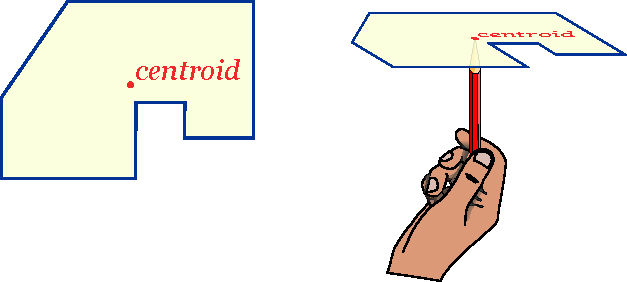
\includegraphics{centroid}
\caption[The centroid.]{The centroid. \footnotemark}
\label{centroid}
\end{figure}
\footnotetext{Image taken from MathIsFun.com.}

Continuing with the new indices we have the accessibility index which is based on the density of sidewalks and roads that make a certain parcel accessible. Given some candidate parcel's service area, the accessibility index is calculated as the total length of sidewalks and roads per square meter. This accessibility is then normalized by dividing it by the accessibility index of the whole area of analysis, which means that a parcel with an accessibility index greater than one is relatively more accessible than the other parcels. Connectivity is an index that measures the connectedness between the candidate parcel and existing nearby facilities, which we can classify into one of two groups: negative and positive facilities\footnote{While I will hereafter refer to facilities that may have perceived negative/positive effects for parks as ``negative/positive facilities", this is by no means a condemnation of any urban facility (except for prisons, we should abolish those).}. So called negative facilities  are ones that could potentially harm the perceived benefits of a park, like morgues and prisons, while positive facilities could be seen to increase the perceived benefits of a park, such as schools and recreational centers. The connectivity index is calculated by subtracting the number of negative facilities from the number of positive facilities within the parcel's service area. So an index greater than zero indicates that a park is expected to capture some extra benefits from the surrounding facilities. This index is purely a count, since there is no information that indicates the relative importance of the externalities provided by each facility, but it could be modified if such information were to become available by including a weight to reflect the importance of the effect of each facility. \\

There is also another aspect of considering nearby facilities which includes weighing them by their proximity. This perspective assumes that the impact of these facilities reduces as their distance from the parcel increases. The closer a facility is to a parcel, then the more it will affect it. As with the previous connectivity index, we subtract the negative facilities from the positive ones. Finally, the cost takes into consideration the potential cost of parcel acquisition as well as the construction costs of the park. This first component is estimated according to real estate appraisals while the second component is calculated based on construction materials, proposed park amenities, park design, operations, and further administrative obligations. \\

While it may not be immediately clear, these considerations are actually going to be the optimization objectives. The decision makers also ranked them in order of importance (a key component of the solution strategy), with the final order being the following:
\begin{enumerate}
\item Maximizing the geographic coverage
\item Maximizing the weighted proximity index
\item Maximizing the number of beneficiaries
\item Maximizing the accessibility index
\item Maximizing the connectivity index
\item Minimizing the cost
\end{enumerate}
We will explore and further explain the mathematical formulations of the six objective functions in order to understand what is happening and then we will proceed to walk through the constraints so we can get a better picture of the entire model. \\

The goal of maximizing the geographic coverage is not too different than the one we presented in our simpler models. In fact, the only difference is that the definition of the service area has changed, as previously discussed. So for the real model we will still have the following as our objective function for the geographic coverage: 
\begin{equation} \label{objective-1}
\textrm{max } f_1 = \sum_{j \in \mathcal{J}} z_j
\end{equation}

We move onto the second objective function which concerns the weighted proximity index. I will first present the mathematical formulation and then we walk through every component of it.
\begin{equation} \label{objective-2}
\textrm{max } f_2 = \sum_{i \in \mathcal{I}}  \left( \sum_{\{k \in \mathcal{E_P}: d_{ik} \leq r^e  \}} \left( 1-\frac{d_{ik}}{r^e} \right) y_i  -   \sum_{\{k \in \mathcal{E_N}: d_{ik} \leq r^e  \}} \left( 1-\frac{d_{ik}}{r^e} \right) y_i   \right)
\end{equation}

Clearly, there is a lot here for us to unpack. What is this objective function attempting to quantify? We are actually trying to measure the externality proximity index, or the impact (positive or negative) of facilities near the park. As described earlier, the further a facility is from a park the less of an effect it will have on said park. So a school across the street from a park will have a much greater impact on the park than a morgue a couple of blocks over. How does this function measure these things? We start by looking at the first term within the parenthesis of the function: $\sum_{\{k \in \mathcal{E_P}: d_{ik} \leq r^e  \}} \left( 1-\frac{d_{ik}}{r^e} \right) y_i$. We start off by defining what certain sets mean. The set $\mathcal{I}$ is the set of all candidate parcels. The set $\mathcal{E}$ defines the set of all urban facilities in the area of analysis (in the town, or region we are considering for this model). Thus, the set $\mathcal{E_P}$ refers to the set of facilities that would have positive effect on a park. The variable $d_{ik}$ refers to the distance from the centroid of candidate parcel $i$ to the facility $k$. The variable $r^e$ defines the maximum distance of effect for any facility. Thus, the term $ \left( 1-\frac{d_{ik}}{r^e} \right) y_i$ indicates as an index the effect from a facility on candidate parcel $i$. We note that the conditions under the summation symbol, $\{k \in \mathcal{E_P}: d_{ik} \leq r^e  \}$ indicate that we are only considering the positive facilities for this term, and only those whose distance to the centroid of the park is within their area of effect. Thus, the term $\sum_{\{k \in \mathcal{E_P}: d_{ik} \leq r^e  \}} \left( 1-\frac{d_{ik}}{r^e} \right) y_i$ indicates that we are measuring the effect of positive facilities on a candidate parcel. Similarly, the term being subtracted, $ \sum_{\{k \in \mathcal{E_N}: d_{ik} \leq r^e  \}} \left( 1-\frac{d_{ik}}{r^e} \right) y_i  $, indicates the effect of negative facilities on a candidate parcel. We note that in this term, we are considering facilities $k \in \mathcal{E_N}$, where $\mathcal{E_N}$ is the set of facilities with negative effect on parks. Thus, subtracting these two terms gives us an index of how positively or negatively affected a park is by the surrounding facilities. Finally, the final summation symbol indicates that we repeat this process for every single candidate parcel. And since we are trying to maximize this objective function, it means that we want to select parcels who will benefit the most from the surrounding facilities' presence. \\

We now move onto the third objective function, where we try to maximize the number of beneficiaries. Again, this is the same as in our model:
\begin{equation} \label{objective-3}
\textrm{max } f_3 = \sum_{i \in \mathcal{I}} p_iy_i
\end{equation}
For a refresher on what this means feel free to turn back to \autoref{changing-objective}. \\ \\
%
We now turn to the accessibility index, which is given by:
\begin{equation} \label{objective-4}
\textrm{max } f_4 = \sum_{i \in \mathcal{I}} v_iy_i
\end{equation}
In this objective function, the variable $v_i$ represent the accessibility index of candidate parcel $i$. As discussed earlier, this is calculated by measuring the total length of sidewalks and roads within the service area of a candidate parcel, and then dividing this measure by the total length of sidewalks and roads over the \textit{entire} area of analysis (the town, city neighborhood, etc). An index greater than one indicates a candidate parcel that is relatively more accessible than the rest.  This is a figure that is calculated for all the candidate parcels, and is something we also try to maximize, because the more accessible a park is, the easier it is for people to go to it! \\

We now consider the connectivity index, which is expressed formulaically as:
\begin{equation} \label{objective-5}
\textrm{max } f_5 = \sum_{i \in \mathcal{I}} e_iy_i
\end{equation}
In this objective function, $e_i$ denotes the connectivity index of parcel $i$. How is this calculated? By looking at the service area of a candidate parcel, we can determine all of the facilities within the service area that may have an impact (positive or negative) on the park. We then take all of the positive facilities within the service area of a parcel and subtract from this number the quantity of negative facilities. So for example, if there are five positive facilities and 3 negative facilities within a parcel's service area, then it would have a connectivity index of two. An index greater than zero might indicate that the park is expected to capture some extra benefits from the surrounding facilities. In fact, this index is related to the weighted proximity index but is slightly different, as it does not take into account the proximity of the facilities and ranks them all as equal, regardless of distance. \\

We can now finally consider the most important objective\footnote{This is a joke.}, where we consider the effect of park-building on our budget. In this objective function, we wish to minimize the costs of our operations:
\begin{equation} \label{objective-6}
\textrm{min } f_6 = \sum_{i \in \mathcal{I}} (c_i^l + c_i^b)y_i
\end{equation}
We have two variables to consider here. The first one, $c_i^l$, indicates the parcel (or lot, hence the $l$) acquisition cost. The second one, $c_i^b$, indicates the cost of building (hence the $b$) a park on parcel $i$. These two variables are measured using real estate appraisals for the former, and material cost, park amenities and design, operations, and other administrative duties. Thankfully, this was ranked as the least important objective to fulfill. Saving money is clearly not the goal here, but if we could be given the choice between building two otherwise identical parks, we might as well choose the less expensive one. Thus it is included as an objective to optimize, but clearly it is not the priority. \\

%
% 2.3.2
%
\subsection{Constraints}
We can now begin to consider what sorts of constraints we might be bounded by. We will first present the constraints that we had already tackled in our simpler model.
\begin{equation} \label{constraint-7}
z_j \leq \sum_{i \in \mathcal{W}_j} y_i \; , \quad j \in \mathcal{J}
\end{equation}
%
\begin{equation} \label{constrain-8}
\left|\mathcal{W}_j\right|z_j \geq \sum_{i \in \mathcal{W}_j} y_i \; , \quad j \in \mathcal{J}
\end{equation}

These constraints guarantee that if a block $j$ is covered, then some parcel covering the block has been selected, and conversely, if block $j$ is not covered, then none of the parcels servicing it should be selected. As a quick refresher, the set $\mathcal{J}$ consists of all the blocks that could benefit from the construction of a park, $z_j$ is a binary valuable indicating whether block $j$ is being serviced or not, and the set $W_j$ is the set of $i$ that could service block $j$. For a more in-depth explanation, please refer back to \autoref{setting-up-problem}. \\

This next constraint indicates that total new park area should meet a minimum requirement.
\begin{equation} \label{constraint-9}
\sum_{i \in \mathcal{I_F}} a_iy_i + \sum_{i \in \mathcal{I_V}} x_i  \geq \underline{a}
\end{equation}
We note that with this constraint, two new sets are introduced: $\mathcal{I_F}$ and $\mathcal{I_V}$. The set $\mathcal{I_F}$ contains the candidate parcels with an area less than or equal to $10000m^2$ (fixed-sized parcels, hence the $\mathcal{F}$ subscript). The other set contains larger parcels, which are referred to as variable-size parcels because the resulting parks built on these candidate parcels may not cover the entire area of the parcel (they might be smaller than the parcel). We note that the union of these two sets is $\mathcal{I}$, our original set. In other words, $\mathcal{I_F} \cup \mathcal{I_V} = \mathcal{I}.$
The variable $a_i$ denotes the area (in square meters) of parcel $i$. Since fixed-size parcels will cover the entire area of their parcel, then we can calculate the area for these resulting parks directly by using the parcel area. For variable sized parcels, however, we let $x_i$ represent the area of candidate parcel $i$ that is to be turned into a park. The variable $\underline{a}$ denotes the minimum requirement for park area as defined by Bogot\'{a}'s recreational master plan (for a reminder of this plan, turn back to \autoref{intro-parks-problem}). \\

On the other hand, we also do not want to build too many parks, because then the IDRD (Recreation and Sports Institute) might be overwhelmed and incapable of administering the excess of parks. Thus, we also implement an upper bound on the amount of parkland we want built:
\begin{equation} \label{constraint-10}
\sum_{i \in \mathcal{I_F}} a_iy_i + \sum_{i \in \mathcal{I_V}} x_i  \leq \bar{a}
\end{equation}
We note this constraint is almost identical to the previous one, with $\bar{a}$ denoting the upper bound for parkland to be built. \\ \\
%
The next constraint puts a size limit on the parks built on variable sized parcels.
\begin{equation} \label{constraint-11}
\underline{s}_iy_i \leq x_i \leq \bar{s_i}y_i \;, \quad i \in \mathcal{I_V}
\end{equation}
The variables $\underline{s}_i$ and $\bar{s_i}$ denote the minimum and maximum construction size parameters for the allotted park area in variable sized parcels. \\ \\
%
We return to familiar constraints, with:
\begin{equation} \label{constraint-12}
y_i \in \{0,1\} \; , \quad i \in \mathcal{I} 
\end{equation}
%
\begin{equation} \label{constraint-13}
z_j \in \{0,1\} \; , \quad j \in \mathcal{J} 
\end{equation}
These constraints define our variables to be binary, as discussed in our simpler model. \\ \\
%
Finally, our last constraint indicates that a variable sized park area cannot be negative (what is negative area?).
\begin{equation}
x_i \geq 0, i \in \mathcal{I_V}
\end{equation}

Put together, the grand model looks like this: 

\begin{figure}
\begin{gather*}
\textrm{max } f_1 = \sum_{j \in \mathcal{J}} z_j \\
\textrm{max } f_2 = \sum_{i \in \mathcal{I}}  \left( \sum_{\{k \in \mathcal{E_P}: d_{ik} \leq r^e  \}} \left( 1-\frac{d_{ik}}{r^e} \right) y_i  -   \sum_{\{k \in \mathcal{E_N}: d_{ik} \leq r^e  \}} \left( 1-\frac{d_{ik}}{r^e} \right) y_i   \right) \\
\textrm{max } f_3 = \sum_{i \in \mathcal{I}} p_iy_i \\
\textrm{max } f_4 = \sum_{i \in \mathcal{I}} v_iy_i \\
\textrm{max } f_5 = \sum_{i \in \mathcal{I}} e_iy_i \\
\textrm{min } f_6 = \sum_{i \in \mathcal{I}} (c_i^l + c_i^b)y_i \\
\textrm{subject to } z_j \leq \sum_{i \in \mathcal{W}_j} y_i \; , \quad j \in \mathcal{J} \\
\left|\mathcal{W}_j\right|z_j \geq \sum_{i \in \mathcal{W}_j} y_i \; , \quad j \in \mathcal{J} \\
\sum_{i \in \mathcal{I_F}} a_iy_i + \sum_{i \in \mathcal{I_V}} x_i \geq \underline{a} \\
\sum_{i \in \mathcal{I_F}} a_iy_i + \sum_{i \in \mathcal{I_V}} x_i \leq \bar{a} \\
\underline{s}_iy_i \leq  x_i \leq \bar{s_i}y_i \;, \quad i \in \mathcal{I_V} \\
y_i \in \{0,1\} \; , \quad i \in \mathcal{I} \\
z_j \in \{0,1\} \; , \quad j \in \mathcal{J} \\
x_i \geq 0 \; , \quad\quad\;\;\; i \in \mathcal{I_V} \\
\end{gather*}
\caption{The grand model}
\label{real-model}
\end{figure}
The one striking difference from the real model compared to our simplified model is that there is no value of $p_{max}$ in the real model. The reason for this is that we are not actually limiting the number of parks to be built, as in our simplified model, but the total area of parkland instead. 
\end{chapter}


%
%
% Chapter 3
%
%
\begin{chapter}{Software and Functions}
We now look at the code that accomplishes what I described in our simplified model in \autoref{complicated-model}. We go through it part by part to understand some of the inner workings. Some previous knowledge of programming and Python (version 3.6.5) is assumed. 

%
% 3.1
%
\section{Programming the Model}
We first take a look at the modules and helper functions that will help us construct and solve our models. \\
\begin{lstlisting}[language = Python, caption = Utilized Python Modules]
import math
import pulp
import re
import ast
\end{lstlisting}
The \textbf{math} module provides access to mathematical functions. Check \href{https://docs.python.org/3/library/math.html}{Python 3.6.5 Documentation} for further information. The \textbf{PuLP} module is a free open source software written in Python and is used to describe optimization problems as mathematical models. It can call numerous external LP solvers and then uses Python commands to describe and display solutions. For more information on this module and for installation procedures turn to the \href{https://pythonhosted.org/PuLP/}{PuLP 1.6.0 Documentation}. The \textbf{re} module provides regular expression matching operations. For more information about this module, refer to the \href{https://docs.python.org/3/library/re.html}{Python 3.6.5 Documentation} as well. We use the \textbf{ast} module to help us evaluate strings containing Python literal structures. Once again, refer to the \href{https://docs.python.org/3/library/ast.html}{Python 3.6.5 Documentation} for more information.\\
In particular, I chose the \textbf{PuLP} library for this project because of its relative ease of use and for its ability to display the formulated linear programs as well as the solutions. We can now move onto more solid chunks of code.\\
\begin{lstlisting}[language = Python, caption = Tells us if two blocks are bordering each other (a proxy for the service area measurement)., xleftmargin = -40pt]
def is_adjacent(block_one, block_two, n, m, adjacent_dist = 1):
	block_one_row = math.ceil(block_one/m)
	block_one_col = block_one % m
	if block_one_col == 0:
		block_one_col = m
	block_two_row = math.ceil(block_two/m)
	block_two_col = block_two % m
	if block_two_col == 0:
		block_two_col = m
	return (math.fabs(block_one_row - block_two_row) 
	<= adjacent_dist and math.fabs(block_one_col - block_two_col) 
	<= adjacent_dist)
	
	
\end{lstlisting} 


This chunk of code takes in several parameters with the aim of determining whether two blocks are adjacent (within their service area), and returns a Boolean (\verb-True- if it's adjacent, \verb-False- if not). It takes the indices of any two blocks, \verb-block_one- and \verb-block_two-, the dimensions of our $\verb-n- \times \verb-m-$ town, and if we wished to we could change the default service area of our parcels from the one to some other value for \verb-adjacent_dist-. Then, based on the given indices of the two blocks, it determines the corresponding row and column for each one by using the town dimensions. It then checks that the two blocks are adjacent by checking that they are at most one row and one column away from each other. Note once again that we can change the the value of \verb-adjacent_dist- to simulate parcels with larger service areas. We express this as a function because we will need to check if two blocks are adjacent to each other numerous times. \\ \\
%
\begin{lstlisting}[language = Python, xleftmargin= -40pt,  caption = Generates the set $\mathcal{J}.$]
def generate_set_j_no_string(candidate_parcels, n, m, pop_dict):
	lots = range(1, (n*m)+1)
	set_j = []
	pop_sum = {}

	for i in candidate_parcels:
		for j in [x for x in lots 
		if x not in candidate_parcels]:
			if is_adjacent(i,j,n,m):
				if i in pop_sum:
					pop_sum[i] = 
					pop_sum[i] + pop_dict[j]
				else:
					pop_sum[i] = pop_dict[j]
				if j not in set_j:
					set_j.append(j)
	return sorted(set_j), pop_sum
\end{lstlisting}
This chunk serves to generate the set $\mathcal{J}$ as well as count the number of beneficiaries that would result from the construction of a park on candidate parcel $i$. It takes as parameters the list of candidate parcels, the dimensions of our model town, and the dictionary that links the blocks to the number of people living on that block. You will note that \verb-pop_sum- is a dictionary with key corresponding to candidate parcel $i$ and whose value stores the number of beneficiaries resulting from the construction of a park on parcel $i$. What we end up doing is that for every candidate parcel, we check \textit{every single lot} that is not a candidate parcel to check whether it is adjacent or not. 

	This is but a na\"{i}ve solution, and it ends up checking a lot of unnecessary lots for adjacency, especially when \verb-adjacent_list = 1- (because when we are only checking for bordering lots, we can have at most eight lots bordering a given lot, but we end up checking every single lot - which could very well be a hundred or so). While we are doing this, however, we also construct the dictionary of candidate parcels and their beneficiaries, as previously mentioned. The time complexity of this algorithm ends up being roughly $O(n^2 \cdot m)$, where $m$ is the number of candidate parcels, and $n$ is the longer dimension of our town. This is due to the set-up of the two for-loops. This function returns the sorted set $\mathcal{J}$ as well as our number of beneficiaries dictionary.\\ \\
%
\begin{lstlisting}[language = Python, caption = Generates the sets $\mathcal{W}_j$ for all $j \in \mathcal{J}$.]
def generate_sets_w(candidate_parcels, n, m, benefitting_sets):
	list_of_w_sets = {}
	w_j = []

	for j in benefitting_sets:
		for i in candidate_parcels:
			if is_adjacent(i,j,n,m):
				if i not in w_j:
					w_j.append(i)
		list_of_w_sets[j] = w_j[:]
		w_j.clear()
	return list_of_w_sets
\end{lstlisting}
This function serves to define the sets $\mathcal{W}_j$, which will contain for a $j \in \mathcal{J}$ all the candidate parcels that serve that block $j$. The outer loop iterates over the lots that could benefit from the construction of a new park (the lots that are in some park's service area), and checks if any candidate parcel is adjacent to them. If so, it adds the candidate parcel to its corresponding $\mathcal{W}_j$ set. It then returns a dictionary, where the key is the lot $j$ and the corresponding value is a list of all the candidate parcels that serve block $j$. \\ \\

\begin{lstlisting}[language = Python, caption = {Appends letter to strings, lists, or dictionaries.}]
def append_letter(letter, num):
	if type(num) is list:
		appended = []
		for n in num:
			appended.append(letter + str(n))
		return appended
	elif type(num) is dict:
		appended = {}
		for key, val in num.items():
			appended[letter + str(key)] = val	
		return appended
	return letter + str(num)
\end{lstlisting}
This helper function simply allows us to append a character to a string, list, or dictionary. If the parameter in \verb-num- is a list or a dictionary, the function will append our given \verb-letter- to every element in the list/dictionary. Otherwise, it will just append the \verb-letter- to the given string. \\ \\

\begin{lstlisting}[language = Python, caption = Helper function using regex]
def extract_num(letters):
	num = (re.search(`\d+', letters))
	return (int(num[0]))
\end{lstlisting}
This smaller function returns the first match of any integer in a string. In other words, it returns the first integer it comes across in a string. So if the input was `1xzr', this function would return 1. We now move onto the meatier part of our program.\\ \\

\begin{lstlisting}[language = Python, caption = Constructs and solves our linear programs., xleftmargin = -50pt]
def solveLP(obj_function, obj_string, 
	candidate_parcels, vars_z, vars_y, 
	max_parks, sets_w, extra_constraint = None):

	# Initialize park location problem
	park_location_model = pulp.LpProblem(
	``Park Location Model: {0}".format(obj_string), pulp.LpMaximize)
	# Add objective function
	park_location_model += obj_function , obj_string

	# Add constraint on maximum number of parks built
	park_location_model += pulp.lpSum(
	[vars_y[y] for y in candidate_parcels]) <= 
	max_parks, ``Can only build {0} park(s)".format(max_parks)


	# add constraints
	for key, val in vars_z.items():
		num = extract_num(key)
		y_constraints = sets_w[num]


		lp_sum = pulp.lpSum([vars_y[y] for y in y_constraints])

 		# these are the conditions of the form
		# z_j <= sum (y_i) for i in W_j
		# followed by the label
		condition_one = lp_sum >= val
		label_one = ``If lot {0} is serviced at 
		least one park is built".format(num)

		# these are the conditions of the form 
		# |W_j| * z_j >= sum(y_i) for i in W_j
		# followed by the label
		condition_two = len(y_constraints) * val >= lp_sum
		label_two = ``If a park serving lot {0} is 
		picked then lot {1} must be serviced".format(num,num)

		# adding both conditions to the model
		park_location_model += condition_one, label_one
		park_location_model += condition_two, label_two

	# Add extra constraint which will be the 
	# deterioration for an objective
	if extra_constraint is not None: 
		park_location_model += extra_constraint , 
		``Objective function deterioration"

	# The problem data is written to an .lp file
	park_location_model.writeLP(``Model-{0}.lp".format(obj_string))

	# The problem is solved using PuLP's choice of Solver
	park_location_model.solve()

	# The status of the solution is printed to the screen
	print (``Status: ", pulp.LpStatus[park_location_model.status])

	blocks_served = 0
	# Each of the variables is printed with its resolved optimum value
	for v in park_location_model.variables():
		print (v.name, ``=", v.varValue)
		if v.name.startswith(`z'):
			blocks_served += v.varValue

	print (``Number of blocks served: {0} ".format(blocks_served))


	# The optimised objective function value is printed to the screen
	print (``{0} = ".format(obj_string), 
	pulp.value(park_location_model.objective))

	return park_location_model	
\end{lstlisting}

\indent	I have included comments in this larger chunk to make it slightly easier to understand. This function takes the parameter \verb-obj_function-, which is the objective function that we are trying to optimize, as well as \verb-obj_string-, which is a short text description of our objective function. It also takes in the set of candidate parcels, the binary variables $z_j$ denoted \verb-vars_z-, the binary variables $y_i$ denoted \verb-vars_y-, and the maximum number of parks we want to build, \verb-max_parks-. When we are in the second stage of our solution strategy, it also takes in \verb-extra_constraint- which is the objective function that we add as a constraint with some compromise threshold, as previously described.

This chunk of code uses \textbf{PuLP} to formulate a mathematical model. It adds the objective function and then the constraint, along with descriptions of them, to our \textbf{PuLP} model. It also outputs the linear program into a file with a \verb-.lp- extension that can be opened in a text editor, so we can verify what our linear program was. It also solves the model, and prints the status of the solution (whether it is optimal or not) to the console. It also then prints out each variable with its corresponding final value in the optimal solution. It then returns this model with all the corresponding information about the optimal solution. \\ \\

\begin{lstlisting}[language = Python, caption = Runs the solution strategy and prints out solutions for many different values of $\alpha_k$., xleftmargin = -50pt]
def place_parks(candidate_parcels, n, m, max_parks, 
	population, lower = 10, upper = 15, step = 5):

	set_j, pop_sum = 
	generate_set_j_no_string(candidate_parcels, n, m, population)
	sets_w = generate_sets_w(candidate_parcels, n, m, set_j)
	set_j = append_letter(`z', set_j)
	
	# forms dictionary of number and variable pairs
	set_i_dict = {}
	for i in candidate_parcels:
		set_i_dict[i] = append_letter(`y', i) 

	# form the variables in the objective function
	vars_z = {}
	vars_y = {}
	for z in set_j:
		vars_z[z] = pulp.LpVariable(
		z, lowBound = 0, upBound = 1, cat = `Integer')
	for key, val in set_i_dict.items():
		vars_y[key] = pulp.LpVariable(
		val, lowBound = 0, upBound = 1, cat = `Integer')

	# putting together the first objective function which
    	# maximizes geographical service area of candidate parcels
	block_objective = ``"
	for key, val in vars_z.items():
		block_objective += val

	# population objective function
	pop_objective = pulp.lpSum(
	vars_y[y] * pop_sum[y] for y in candidate_parcels)

	# Setting up LP and solving it for servie area objective
	print(``Solving in isolation for service area objective function\n")
	LP1 = solveLP(block_objective, 
		``Maximum number of blocks serviced", candidate_parcels, 
		vars_z, vars_y, max_parks, sets_w)

	LP1_obj_value = pulp.value(LP1.objective)

	# Setting up new LP and solving it for population objective
	print(``Solving in isolation for population objective function\n")
	LP2 = solveLP(pop_objective, 
		``Maximum number of beneficiaries", candidate_parcels, 
		vars_z, vars_y, max_parks, sets_w)

	for i in range(lower, upper, step):
		# maximum acceptable deterioration amount
		det_amount = i / 100
		deterioration = LP1.objective >= 
		(1 - det_amount) * LP1_obj_value
		
		# solving both objectives
		print(``Solving both objective functions\n")
		print(``Acceptable deterioration value: {0}%".format(i))
		LP3 = solveLP(pop_objective, 
			``Maximizing beneficiaries 
			considering blocks serviced", 
			candidate_parcels, vars_z, vars_y, 
			max_parks, sets_w, deterioration)
\end{lstlisting}
	I again have included comments to facilitate the understanding of this chunk of code. This function takes in several parameters. It takes in the set (list) of candidate parcels, the dimensions of our model town, and the maximum number of parks we wish to build. It also requires a variable \verb-population-, which is the population dictionary with block indices as keys and the population living on that block as the value pairing. 
	
	The variables \verb-lower-, \verb-upper-, and \verb-step- are all concerned with our model variable of $\alpha_k$. The variable \verb-lower- is concerned with the minimum allowable deterioration we decide to try. It is given as a percentage in our program, so it would range from 0 to some value less than 100. Similarly, \verb-upper- is the maximum allowable deterioration decided upon by the decision maker. It must be greater than \verb-lower-. Finally, \verb-step- denotes the intervals at which we wish to try values of $\alpha_k$. For example, if we let $\verb-lower- = 0$, $\verb-upper- =20$, and $\verb-step-=5$, then for the second stage of our solution strategy (optimizing with the added objective constraint), it will solve our model for $\alpha_k = 0,5,10,15,20$. We can then have a better idea of what our options are, and potentially hone in on an optimal answer. 
	
	You'll note that the first few lines in this function are dedicated to generating the necessary sets in a way that we can work with. We generate our set $\mathcal{J}$, the necessary $\mathcal{W}_j$ sets, and we also establish a link between the indices $i$ and their corresponding $y_i$ variable. In the variables \verb-vars_z- and \verb-vars_y- we form the corresponding \verb-pulp.LpVariable- for each set of variables $z_j$ and $y_i$. We then set up our two objective functions and solve the linear programs in isolation (step one of our solution strategy). Afterwards, we use the variables \verb-lower-, \verb-upper-, and \verb-step- to perform the second stage of our solution strategy and attempt to find an optimal solution. \\ \\ \\

	We have now presented our problem, worked through increasingly complicated models, and explored the technical aspects of our work. We can now conclude this exercise, hoping that Operations Research will continue to find even greater application as a tool for demanding equity and bringing about meaningful social change, even if it does so in seemingly unimpressive ways -- like optimizing the placement of public parks in a city. With that being said: if you have been, thanks for listening!
\end{chapter}

\bibliographystyle{ieeetr}
\bibliography{final-bib}

\end{document}

 